\documentclass{article}
\usepackage{nips07submit_e,times}
%\documentstyle[nips07submit_09,times]{article}
\usepackage{graphicx}
\usepackage{subfigure}
\usepackage{amssymb}

\title{Infinitely-Armed Bandit Algorithms}


\author{
Matthew Faulkner\\
\\
\And
Jon Krause \\
\\
\And
Daniel Rosenberg \\
\\
}

% The \author macro works with any number of authors. There are two commands
% used to separate the names and addresses of multiple authors: \And and \AND.
%
% Using \And between authors leaves it to \LaTeX{} to determine where to break
% the lines. Using \AND forces a linebreak at that point. So, if \LaTeX{}
% puts 3 of 4 authors names on the first line, and the last on the second
% line, try using \AND instead of \And before the third author name.

\newcommand{\fix}{\marginpar{FIX}}
\newcommand{\new}{\marginpar{NEW}}

\begin{document}

%\makeanontitle
\maketitle

\begin{abstract}
We have been considering a variation on the standard K-armed bandit 
problem where the number of arms is infinite.  Here we present
our progress and plans for the future.
\end{abstract}

\section{Background}
In many situations, the number of arms on a K-armed bandit is actually
very large.  For example, in the case of choosing an ordering of $N$ ads,
the number of possible arms to pull is actually $N!$, which is far too
large for any standard finite-armed bandit algorithm to handle.
Generalizing, it may be the case that the number of arms on a bandit is
actually infinite.  Examples of this include optimizing parameters of
some algorithm or classifier and maximizing a noisy function over a domain
containing an infinite number of points, such as a unit hypercube.

The algorithms designed to handle an infinite-armed bandit can be
partitioned into those algorithms which merely discretize the domain
into a finite number of points, and those which actually take into
consideration every point.  One natural question to ask is: are these
infinite-armed bandit algorithms worth it, or is it more advantageous
to stick with a discretization of the domain into a finite number of
points and run a standard finite-armed bandit algorithm on them?
With that in mind, we implemented the following algorithms: discretized
UCB1, discretized $\epsilon$-greedy, discretized Exp3,
Zooming\cite{Zooming}, and
Hierarchical Optimistic Optimization (HOO)\cite{xArmed}.
The latter two of these
algorithms are designed to work on an infinite-armed bandit, whereas the
former three all pick a finite number of points in the domain to run on.


\section{Algorithms}
\subsection{General Framework}
The first order of business in implementing any of these algorithms was
abstracting everything out so that they could all be easily applied
without too much redundant code.  For example, the HOO algorithm works
on reward functions over topological spaces, and the Zooming algorithm
works on reward functions over metric spaces, so ideally we should just
be able to pass in some domain that the problem is over and the algorithm
should just be able to work.  This is what we have done.  In addition,
bandits have been abstracted (see section on artificial data).


\subsection{Discretization Algorithms}
The simplest approach that one can take when tackling an infinite number of
arms is to merely pick out some finite number of arms and run a standard
finite-armed bandit algorithm on them.  This raises the following 
questions:
\begin{itemize}
\item How many arms should be chosen?
\item How should the arms be chosen?
\end{itemize}
The answer to the first question is algorithm- and problem-specific.  For
example, consider the case where the reward function $r(x) = x$ defined
on the interval $[0,1]$.  With no noise, the $\epsilon$-greedy strategy
will converge to the correct arm immediately after sampling each arm once,
and thus it is beneficial to choose a very large number of arms.  A
UCB1 or Exp3 strategy, though, will take significantly longer to
converge, so if convergence time is an issue, perhaps fewer arms should be
chosen at the expense of some accuracy.  On the other hand, for a
needle-in-a-haystack type of reward function, we clearly want to
include more arms so that we have a better chance of achieving the
optimal value.

Concerning how the arms themselves are chosen, two obvious strategies are
to either choose them randomly or to choose them in a grid (at regular
intervals in the 1D case).  Choosing the arms in a deterministic way
means that, for a fixed number of arms, we can construct a reward function
that makes the algorithm behave terribly.  Even given an arbitrary number
of arms, by choosing a reward function with a maximum near an endpoint of
an interval in $\mathbb{R}$, for example, we can ensure that the algorithm
would never do too well.  For these reasons, we opt to go with a random
choice of arms.

In any case, merely discretizing the domain into a finite number of arms
introduces a bias, as our effective hypothesis class (each of the arms)
probably no longer contains the optimal hypothesis.

\subsection{Zooming Algorithm}
If you actually want to consider the infinite number of arms, you need
to have certain information about the relationship between them. For
instance, arms that are \emph{close} should produce similar
results. The Zooming Algorithm is defined to work in any example where
the arms form a metric space. In each phase, certain arms are chosen
to be \emph{active}, and the algorithm chooses which arm to play from
these active arms.

The Zooming Algorithm is composed of multiple phases, each of which is
composed of $2^{i_{ph}}$ rounds, where $i_{ph}$ is the current phase
number. In a given round, you \emph{activate} an arm if that arm is
not covered by another arm. Each arm covers a radius defined by
$r_t(v):=\sqrt{8*i_{ph}/(2+n_t(v)))}$ where $v$ is the active arm, and
$n_t(v)$ is the number of times a given arm has been chosen at time
$t$. Each time an arm is played, its radius shrinks, and at the
beginning of each round, you \emph{activate} arms until you have a
complete covering using a \emph{covering oracle}. This oracle can
either return an uncovered arm, or state that there is no such
arm. After the space is covered, you play the arm with the optimal
index, defined as $I_t(v):=\mu_t(v)+2*r_t(v)$

A point of concern to us with this algorithm is that it does not seem
to remember anything from previous phases when a new phase starts. The
only piece of information it maintains is the phase number, which
influences the confidence radius and index, which changes the balance
between exploration and exploitation. It seems like it may be better
to start on a later phase, given knowledge of the specific
problem. Additionally, the \emph{covering oracle} becomes very
complicated once you move into more advanced spaces.

Additionally, we have run into some issues under more complicated
bandit problems. When there are multiple peaks, the algorithm seems to
have trouble converging. This may be due to a bug in our code, or some
parameter that needs to be tuned in the algorithm.

\subsection{Hierarchical Optimistic Optimization}
Our final algorithm addresses the case of infinite arms over an
arbitrary topological space $X$. The hierarchical optimistic
optimization algorithm (HOO) applies to this case under several
assumptions. First, the payoffs are stochastic (non-adversarial), with
distributions of bounded support. Second, the payoff function mapping
arms in $X$ to rewards is \emph{weakly Lipschitz}, which in short requires
the function to be Lipschitz at any maxima, but does not constrain the
function at points away from a maxima.
\\
The HOO algorithm is implemented by iteratively refining a
\emph{covering tree} over $X$, and maintaining confidence bounds
for each node in the tree. The covering tree is a binary tree where
each node represents (covers) a subset of $X$ equal to the union of
all subsets of nodes beneath it in the tree. Whenever the algorithm
selects an arm, a new leaf containing that arm is added to the
tree. The region covered by a new leaf is a subset of the region
covered by its parent, so in this way the leaves define an increasing
fine cover of $X$. For each node $n_i$ in the tree, an empirical
average $\mu_i$ of all rewards received by arms covered by node $n_i$
is maintained, along with an upper confidence bound for
$\mu_i$. These upper confidence bounds are used whenever the algorithm
selects an arm: roughly, the algorithm descends the tree by choosing
at each node the child with larger upper confidence bound. In this
way, HOO resembles the UCB1 algorithm for gaussian processes, in that
nearby points have similar confidence bounds, and that the algorithm
optimistically selects using these bounds.

So far, the HOO algorithm has been implemented using a covering tree
on the unit hypercube for a Euclidean space. This is specifically
analyzed in \cite{xArmed}. While this is a suitable space for many
experiments, we are also considering implementing a more specifically
``topological'' space, such as a torus, which would involve a similarly
implemented covering tree, but would allow evaluation of the
algorithm on a more interesting space.
\\
\section{Artificial Data}
For now, we have just been testing the algorithms on reward functions from
$[0,1]$ to $\mathbb{R}$.  We currently have support for polynomials
of arbitrary degree, binomial functions, composing two arbitrary functions,
and adding noise in the form of multiplying the unbiased result by a random
number in a given range.

\section{Possible Applications}
One issue with bandit algorithms is that there are relatively few
situations where a pure bandit algorithm is applicable.  Rather, is it
typically the case that there is some side information (e.g. a search
term) that can be used in determining which arm to choose.  In that
case, this turns into a contextual bandit problem, which the
algorithms we have implemented are not suited for.  It might be
possible to adapt these algorithms for the contextual bandit problem,
but that would appear to be a project in and of itself.  \\
\section{Conclusion}
In conclusion, we did some stuff, and will do more.
\\
\section{Future Work}
In the next month or so, we intend to add more domains that our algorithms
can work over.  This should be relatively easy due to the abstraction
as described above, although certain aspects might be difficult (i.e.
constructing a covering oracle).  We would also like to move beyond
artificial data.  One possibility is applying these algorithms to
locations of a set of sensors.  While there is real data available for 
this, the data is naturally only taken at a finite number of locations
or configurations, and so we would have to interpolate this data to come
up with a reward function defined over all possible positions.

Another possibility is applying these algorithms to parameters in other
algorithms.  For example, when designing an AI for say, Tic-Tac-Toe, 
we might have a scoring function on a given board describing how
`good' that board is for the current player, and play the move that gives
us the highest score.  One (not necessarily optimal)
way to implement this scoring function would be to assign a weight to each
square on the board, and score the board by the weight of each position
combined with which player occupies each position.  Here, one of our
bandit algorithms could be used to determine the optimal set of weights
to use.  Since these algorithms do not necessarily work against an
adversary, though, we would have to have them play against a random
player.

Going back to artificial data, we could also try to construct reward
functions that cause certain algorithms to do well and others to do poorly.
This would be proof that no algorithm is necessarily better than the others
in all cases, and would answer our initial ``Is it worth it?'' question.
We could also attempt to improve the Zooming algorithm so that information
is carried over between the different phases, make or own experimental
algorithms, or implement more algorithms from more papers.  At this
point, we have not decided for sure which of these options we would like
to pursue, which is also dependent on how much time they take up.

\section{Plots}
The following plots were based on the reward function
$R(x) = noise(bin(3x^2 -3x + 1), .5, 1)$, where $noise(f(x), a, b)$
multiplies each value received from f(x) by some number chosen uniformly
at random between $a$ and $b$, and $bin(f(x))$ is 1 with probability
f(x) and 0 otherwise.  Our implementation of the $\epsilon$-greedy 
algorithm samples each arm once at first, then proceeds with
$\epsilon$ = $\frac{arms}{rounds}$.  The Exp3 algorithm uses
$\gamma = \frac{arms}{rounds + 1}$.  In each discretization case, 100
arms were used.

\newcommand{\figwidth}{5in}
%% \begin{figure}[ht]
%%  \begin{minipage}[b]{.5\linewidth}
%%  \centering
%%  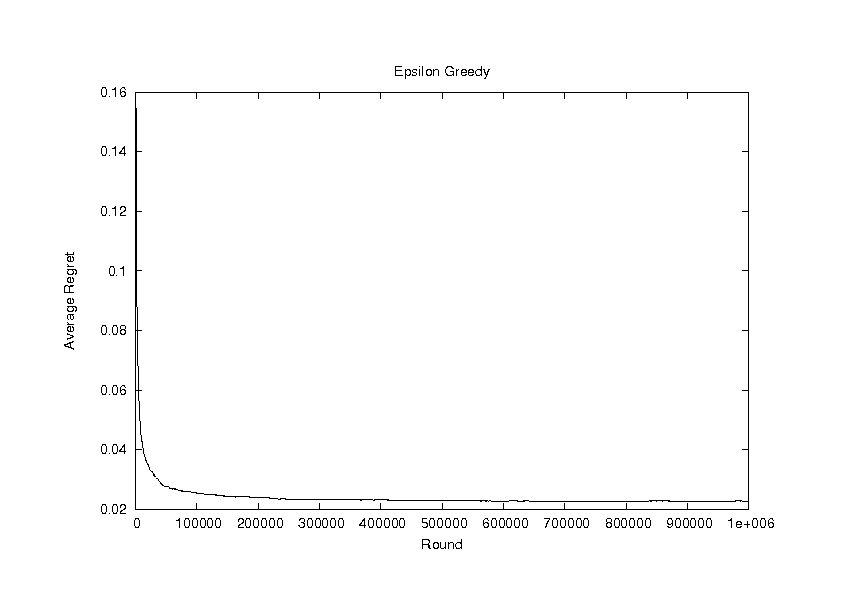
\includegraphics[width=\figwidth]{images/e_greed.png}
%%  % image.png: 480x480 pixel, 72dpi, 16.93x16.93 cm, bb=0 0 480 480\
%%  \caption{Epsilon Greedy}
%%  \label{e_greed}
%%  \end{minipage}
%%  \begin{minipage}[b]{.5\linewidth}
%%  \centering
%%  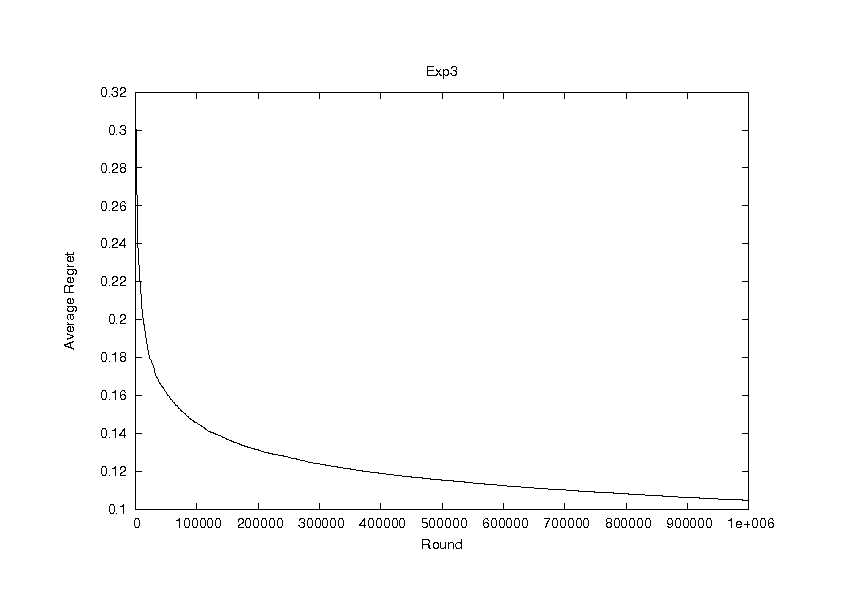
\includegraphics[width=\figwidth]{images/exp3.png}
%%  % image.png: 480x480 pixel, 72dpi, 16.93x16.93 cm, bb=0 0 480 480\
%%  \caption{Exp3}
%%  \label{exp3}
%%  \end{minipage}
%% \end{figure}

%% \begin{figure}[ht]
%%  \begin{minipage}[b]{.5\linewidth}
%%  \centering
%%  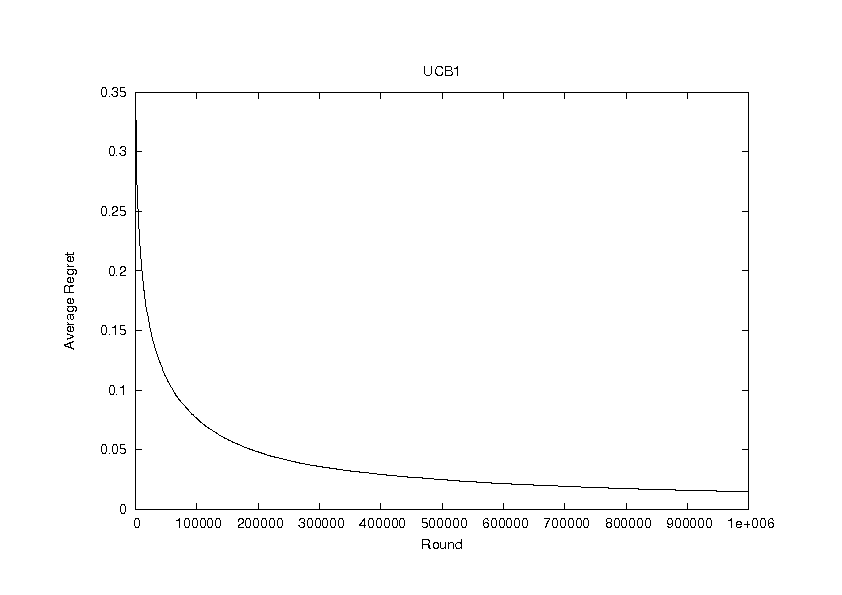
\includegraphics[width=\figwidth]{images/ucb1.png}
%%  % image.png: 480x480 pixel, 72dpi, 16.93x16.93 cm, bb=0 0 480 480\
%%  \caption{UCB1}
%%  \label{ucb1}
%%  \end{minipage}
%% \end{figure}

\begin{figure}[htb]
  \begin{center}
    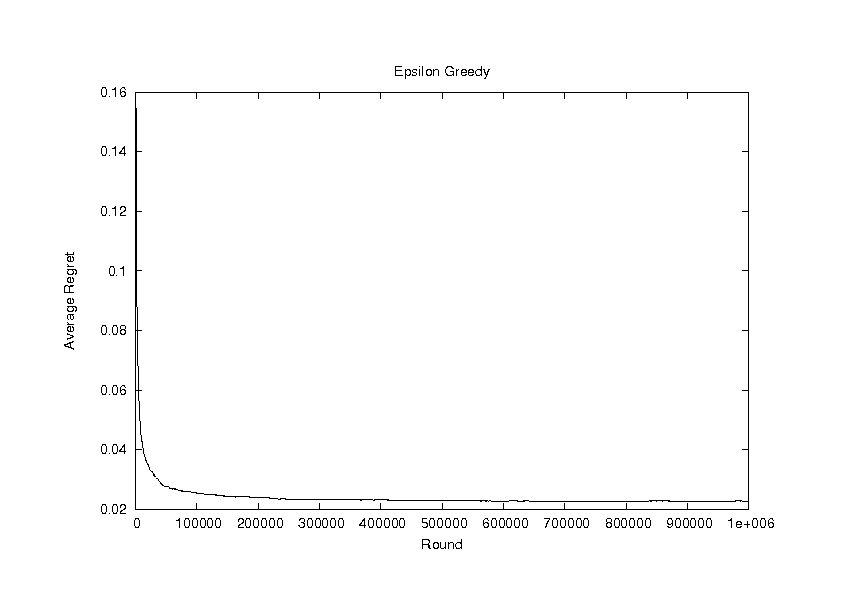
\includegraphics[width=\figwidth]{images/e_greed.png}
     \caption{$\epsilon$ greedy}
     \label{fig:egreed}
  \end{center}
\end{figure}

\begin{figure}[htb]
  \begin{center}
     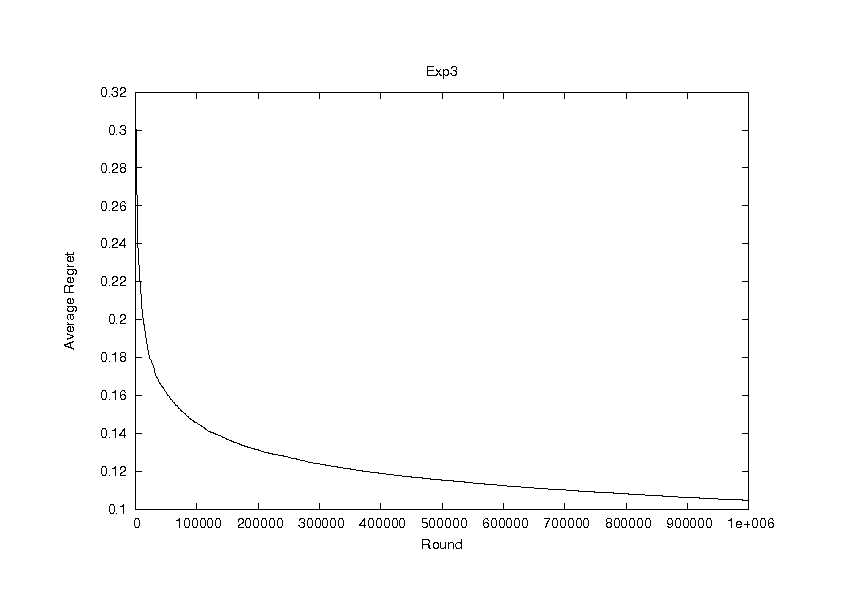
\includegraphics[width=\figwidth]{images/exp3.png}
     \caption{EXP3}
     \label{fig:exp3}
  \end{center}
\end{figure}

\begin{figure}[htb]
  \begin{center}
     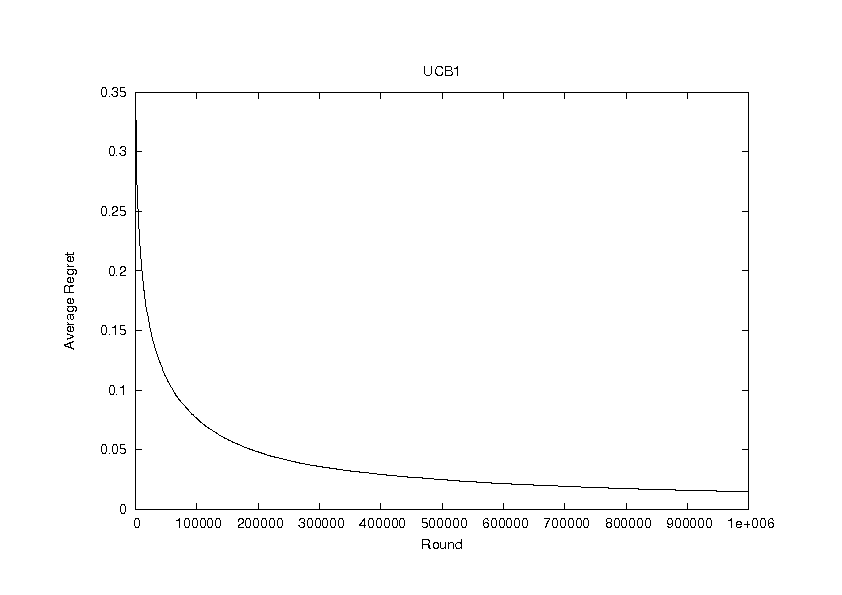
\includegraphics[width=\figwidth]{images/ucb1.png}
     \caption{Discretized UCB1}
     \label{fig:ucb1}
  \end{center}
\end{figure}

\begin{figure}[htb]
  \begin{center}
     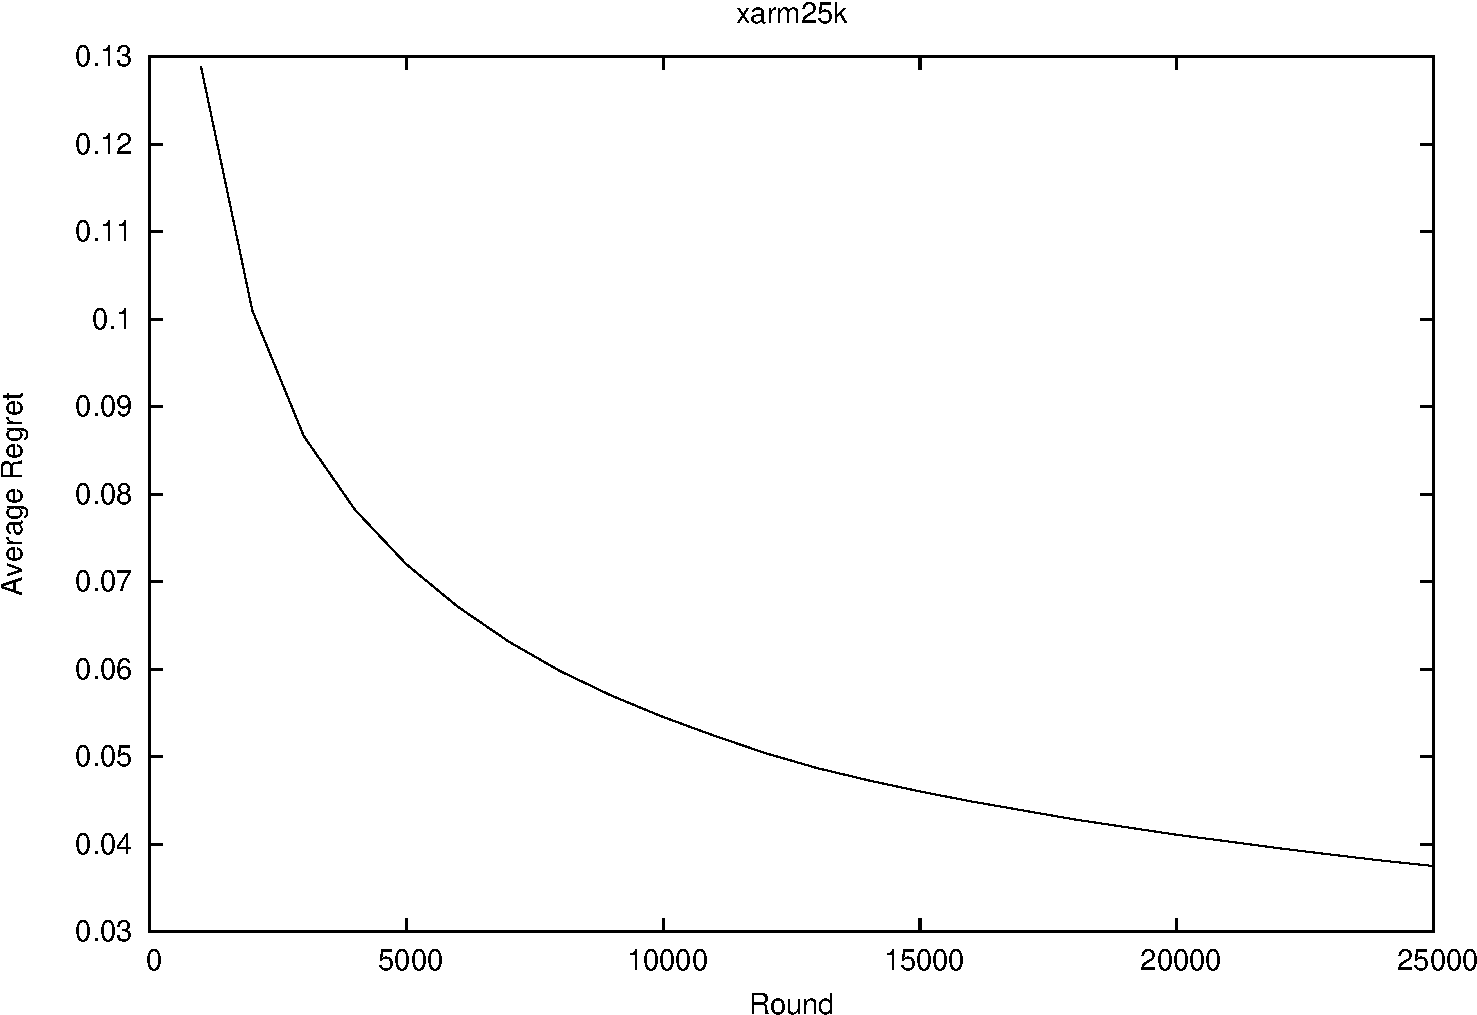
\includegraphics[width=\figwidth]{images/xarm25k-crop.pdf}
     \caption{HOO algorithm regret.}
     \label{fig:hoo}
  \end{center}
\end{figure}


All of our code is available at:
\begin{verbatim}
http://code.google.com/p/bandits/
\end{verbatim}



% References
\begin{thebibliography}{99}

\bibitem{xArmed}S. Bubeck, R. Munos, G. Stoltz, and C. Szepesvari.
``Online Optimization in $\chi$-Armed Bandits''.
\emph{Advances in Neural Information Processing Systems 21}, 2009, pp. 201-208.

\bibitem{Zooming}R. Kleinberg, A. Slivkins, and E. Upfal.
``Multi-Armed Bandits in Metric Spaces''.
\emph{Proceedings of the 40th ACM Symposium on Theory of Computing}, 2008.

\end{thebibliography}
\end{document}
